% Native editable figure; frozen statistics 0d291b4aebf8c524dc6705d872c070feb990e86a1cebbd59a758f400b240c952
\begin{minipage}[t]{.32\linewidth}\centering
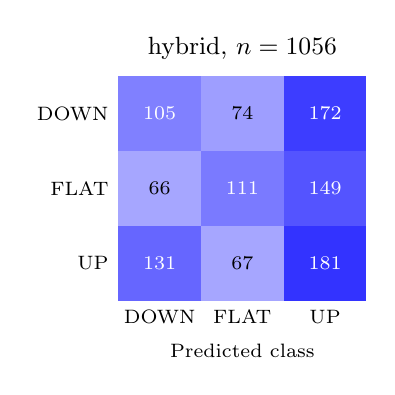
\begin{tikzpicture}[x=1.05cm,y=.95cm,font=\scriptsize]
\fill[blue!50] (0,2) rectangle ++(1,1);\node[text=white] at (0.5,2.5) {105};
\fill[blue!38] (1,2) rectangle ++(1,1);\node[text=black] at (1.5,2.5) {74};
\fill[blue!76] (2,2) rectangle ++(1,1);\node[text=white] at (2.5,2.5) {172};
\fill[blue!35] (0,1) rectangle ++(1,1);\node[text=black] at (0.5,1.5) {66};
\fill[blue!52] (1,1) rectangle ++(1,1);\node[text=white] at (1.5,1.5) {111};
\fill[blue!67] (2,1) rectangle ++(1,1);\node[text=white] at (2.5,1.5) {149};
\fill[blue!60] (0,0) rectangle ++(1,1);\node[text=white] at (0.5,0.5) {131};
\fill[blue!35] (1,0) rectangle ++(1,1);\node[text=black] at (1.5,0.5) {67};
\fill[blue!80] (2,0) rectangle ++(1,1);\node[text=white] at (2.5,0.5) {181};
\node[below] at (0.5,0) {DOWN};\node[left] at (0,2.5) {DOWN};
\node[below] at (1.5,0) {FLAT};\node[left] at (0,1.5) {FLAT};
\node[below] at (2.5,0) {UP};\node[left] at (0,0.5) {UP};
\node[above,font=\small] at (1.5,3.1) {hybrid, $n=1056$};
\node[below] at (1.5,-.45) {Predicted class};\end{tikzpicture}\end{minipage}
\hfill
\begin{minipage}[t]{.32\linewidth}\centering
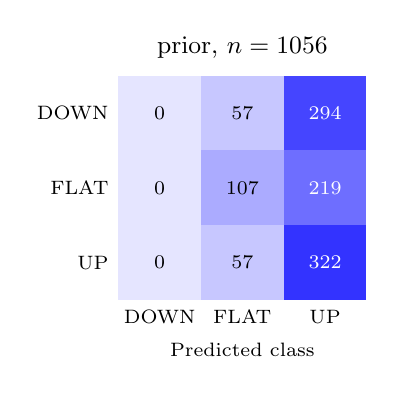
\begin{tikzpicture}[x=1.05cm,y=.95cm,font=\scriptsize]
\fill[blue!10] (0,2) rectangle ++(1,1);\node[text=black] at (0.5,2.5) {0};
\fill[blue!22] (1,2) rectangle ++(1,1);\node[text=black] at (1.5,2.5) {57};
\fill[blue!73] (2,2) rectangle ++(1,1);\node[text=white] at (2.5,2.5) {294};
\fill[blue!10] (0,1) rectangle ++(1,1);\node[text=black] at (0.5,1.5) {0};
\fill[blue!33] (1,1) rectangle ++(1,1);\node[text=black] at (1.5,1.5) {107};
\fill[blue!57] (2,1) rectangle ++(1,1);\node[text=white] at (2.5,1.5) {219};
\fill[blue!10] (0,0) rectangle ++(1,1);\node[text=black] at (0.5,0.5) {0};
\fill[blue!22] (1,0) rectangle ++(1,1);\node[text=black] at (1.5,0.5) {57};
\fill[blue!80] (2,0) rectangle ++(1,1);\node[text=white] at (2.5,0.5) {322};
\node[below] at (0.5,0) {DOWN};\node[left] at (0,2.5) {DOWN};
\node[below] at (1.5,0) {FLAT};\node[left] at (0,1.5) {FLAT};
\node[below] at (2.5,0) {UP};\node[left] at (0,0.5) {UP};
\node[above,font=\small] at (1.5,3.1) {prior, $n=1056$};
\node[below] at (1.5,-.45) {Predicted class};\end{tikzpicture}\end{minipage}
\hfill
\begin{minipage}[t]{.32\linewidth}\centering
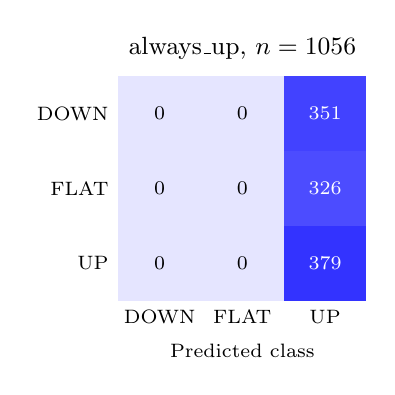
\begin{tikzpicture}[x=1.05cm,y=.95cm,font=\scriptsize]
\fill[blue!10] (0,2) rectangle ++(1,1);\node[text=black] at (0.5,2.5) {0};
\fill[blue!10] (1,2) rectangle ++(1,1);\node[text=black] at (1.5,2.5) {0};
\fill[blue!74] (2,2) rectangle ++(1,1);\node[text=white] at (2.5,2.5) {351};
\fill[blue!10] (0,1) rectangle ++(1,1);\node[text=black] at (0.5,1.5) {0};
\fill[blue!10] (1,1) rectangle ++(1,1);\node[text=black] at (1.5,1.5) {0};
\fill[blue!70] (2,1) rectangle ++(1,1);\node[text=white] at (2.5,1.5) {326};
\fill[blue!10] (0,0) rectangle ++(1,1);\node[text=black] at (0.5,0.5) {0};
\fill[blue!10] (1,0) rectangle ++(1,1);\node[text=black] at (1.5,0.5) {0};
\fill[blue!80] (2,0) rectangle ++(1,1);\node[text=white] at (2.5,0.5) {379};
\node[below] at (0.5,0) {DOWN};\node[left] at (0,2.5) {DOWN};
\node[below] at (1.5,0) {FLAT};\node[left] at (0,1.5) {FLAT};
\node[below] at (2.5,0) {UP};\node[left] at (0,0.5) {UP};
\node[above,font=\small] at (1.5,3.1) {always\_up, $n=1056$};
\node[below] at (1.5,-.45) {Predicted class};\end{tikzpicture}\end{minipage}